\section{Mutex watershed}~\label{sec:mtx_wtsd}
The Mutex Watershed algortihm introduced in \cite{wolf2019mutex} is a image partitioning algorithm based on watersheding that is able to operate without a prior seeding.\\
Like most image partitioning algorithms it is defined on a graph $G=(V, E^+ \cup E^-, W^+ \cup W^-)$ with a set of vertices $V$, a set of edges as the disjoint union of attractive edges $E^+$ and repulsive edges $E^-$ and a set of corresponding edge weights $ W^+ \cup W^-$. Each vertex in this graph represents uniquely a pixel in the corresponding image. The edge weights are based on the affinity between the incidental vertices the respective edge. The affinity between two nodes $i$ and $j$ is the probability $p_{ij}$ of the nodes belonging to the same partition in the posterior partitioning. These affinities can be based on differences in pixel intesities or be predicted by e.g. a CNN. \\
Attractive edges $e_{ij}^+ \in E$ have edge weights $w_{ij}^+ \in W$ with $w_{ij}^+ = p_{ij}$. Repulsive edges $e_{ij}^- \in E$ have edge weights $w_{ij}^- \in W$ with $w_{ij}^- = 1-p_{ij}$. \\
A partitioning on $G$ is defined by the disjoint union of a set of attracive and a set of repulsive edges by the active set $A=A^+ \cup A^-$ that encode hard merges and mutual exclusions of vertices and partitions. To represent a valid partitioning, the set $A$ has to satisfy cycle constraints. Defining the set $\mathcal{C}_i(A)$  with $A\subseteq E$ as the set of all cycles with exactly $i$ active repulsive edges
\begin{align}
	\mathcal{C}_i(A) := \left\{ c \in cycles(G) \vert c \subseteq A \text{  and  } |c \cap E^- | = i \right\},
\end{align}
a valid partitioning can only be inferred from an active set $A$ if $\mathcal{C}_1(A) = \emptyset $. If additionally $\mathcal{C}_0(A) = \emptyset $, the algorithm can be defined as the search for the minimal spanning tree in each partition.\\
\vspace{8mm}\\
\begin{algorithm}[H]
	\KwData{weighted graph $G=(V, E^+ \cup E^-, W^+ \cup W^-)$}
	\KwResult{clusters defined by spanning forest $A^\star \cap E^+$}
	Initialization: $A = \emptyset$\;
	\For{$(i, j) = e \in(E^+ \cup E^-)$ in descending order of $W^+ \cup W^-$}{
		\If{$\mathcal{C}_0(A \cup \{ e \}) = \emptyset$ and  $\mathcal{C}_1(A \cup \{ e \}) = \emptyset$}{
			$A \leftarrow A \cup e$ \;
		}
	}
	$A^\star \leftarrow A$ \;
	\Return $A^\star$
	\caption{Mutex Watershed \cite{wolf2019mutex}}
	\label{algo:mtx_wtsd}
\end{algorithm}
\vspace{8mm}

An example walk through of the algorithm is depicted in figure \ref{fig_mtxwtsd1}. \\

\begin{figure}
	\centering
	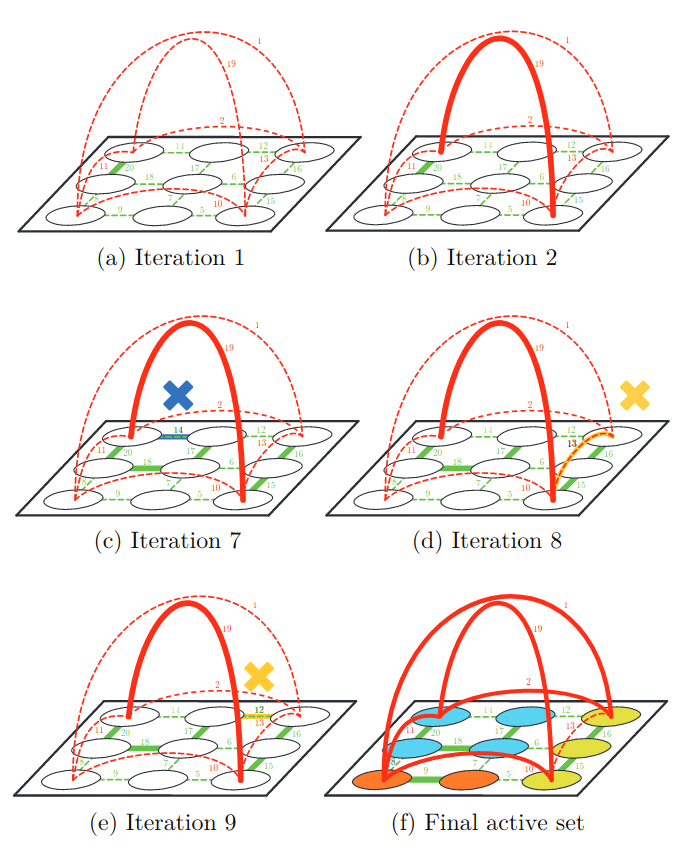
\includegraphics[width=0.5\textwidth]{figures/mutexwatershed/walkthrough}
	\caption{\cite{wolf2019mutex} Some iterations of algorithm \ref{algo:mtx_wtsd} applied to a graph with weighted attractive edges (green) and repulsive (red) edges. Edges that are part of the active set $A$ at each iteration are shown in bold. On termination (f), the connected components in $A \cap E^+$ represent the partitions of the final partitioning. Edges that are not added to $A$ because of the violation of $\mathcal{C}_0$ or $\mathcal{C}_1$ are highlighted in blue and yellow respectively.}
	\label{fig_mtxwtsd1}
\end{figure}

\newpage
Algorithm \ref{algo:mtx_wtsd} minimizes a energy functional that is defined by the active set $A$. This requires the following definition
\begin{defn}
	\textbf{Dominant power} \cite{wolf2019mutex}: \\
	Let $G = (V, E, W)$ be an edge weighted graph, with unique edge weights $w_e \in \mathbb{R}_0^+$, $\forall e \in E$. Then $p \in \mathbb{R}^+$ is called a dominant power if:\\
	\begin{align}
		w_e^p > \sum_{\substack{t \in E \\ w_t < w_e}} w_t^p \text{\hspace{8mm},} \forall e \in E
	\end{align}
\end{defn}
 This allows the definition of the objective that is solved by algorithm \ref{algo:mtx_wtsd}
 
 \begin{defn}
 	\textbf{Mutex Watershed Objective} \cite{wolf2019mutex}: \\
 	Let $G = (V, E, W)$ be an edge weighted graph, with unique edge weights $w_e \in \mathbb{R}_0^+$, $\forall e \in E$ and $p \in \mathbb{R}^+$ a dominant power. Then the Mutex Watershed Objective is devined as the integer linear program:\\
 	\begin{align}
 		\min_{a\in {0,1}^{|E|}} - \sum_{e \in E} a_e w_e^p \\
		\text{s.t. \hspace{2mm}} \mathcal{C}_0(A) = \mathcal{C_1}(A) = \emptyset \text{, }\\
		\text{with \hspace{2mm}} A := \{ e \in E|a_e = 1 \}
 	\end{align}
 \end{defn}
